\documentclass[titlepage, a4paper]{article}
\usepackage[english]{babel}
\usepackage[utf8]{inputenc}
\usepackage{graphicx}
\usepackage{color}
\usepackage{mathtools}
\usepackage{float}
\usepackage[parfill]{parskip}
\usepackage[margin=10pt,font=small,labelfont=bf,labelsep=endash]{caption}
\usepackage{epstopdf}
\usepackage{listings}
\usepackage[table]{xcolor}
\usepackage{tabularx}
\usepackage{colortbl}
\epstopdfsetup{suffix=}
\DeclareGraphicsExtensions{.ps}
\DeclareGraphicsRule{.ps}{pdf}{.pdf}{`ps2pdf -dEPSCrop -dNOSAFER #1 \noexpand\OutputFile}
\usepackage{tikz}
\usetikzlibrary{arrows}

\definecolor{green}{rgb}{56,90,115}

\makeatletter
\def\minuscellcolor{%
  % \ignorespaces not really needed, because \@ifnextchar gobbles spaces
  \@ifnextchar.{\cellcolor{red}}{}%
}
\newcolumntype{C}{>{\minuscellcolor}r}
\makeatother

\lstset{literate=%
    {å}{{\r{a}}}1
    {ä}{{\"a}}1
    {ö}{{\"o}}1
    {Å}{{\r{A}}}1
    {Ä}{{\"A}}1
    {Ö}{{\"O}}1
}

\newcommand{\todo}[1] {\textbf{\textcolor{red}{#1}}}

\usepackage{fancyhdr}
\fancyhead[L]{}
\pagestyle{fancy}
\rhead{Alexander Yngve \\ Pål Kastman}
\chead{TDTS08}
\thispagestyle{empty}

\begin{document}

{\ }\vspace{45mm}

\begin{center}
  \Huge \textbf{TDTS08: Lab Report}
\end{center}
\begin{center}
  \Large Lab 4: VLIW Processors
\end{center}

\vspace{250pt}

\begin{center}
  \begin{tabular}{|*{3}{p{40mm}|}}
    \hline
    \textbf{Name} & \textbf{PIN} & \textbf{Email} \\ \hline
           {Alexander Yngve} & {930320-6651} & {aleyn573@student.liu.se} \\ \hline
           {Pål Kastman} & {851212-7575} & {palka285@student.liu.se} \\ \hline
  \end{tabular}
\end{center}
\newpage

\tableofcontents
\thispagestyle{empty}
\newpage

\section{Introduction}\label{sec:intro}
The purpose of this lab was to convert normal sequential code to VLIW instructions, so that we would get a greater performance. Basically we do what the VLIW compiler does during compilation time.
\section{Method}
The approach for this lab was the following:

\begin{enumerate}
\item Choose a basic block, and disassemble the block. 
\item Find dependencies between the instruction in the block.
\item We pack the instruction into VLIWs.  
\end{enumerate}

\subsection{Basic Block}\label{sec:bb}
To view all the basic blocks within the program (go.ss) the following command is issued:

\begin{lstlisting}
vliwc /home/TDTS08/bin/go.ss | sort -nr +3 -4 | less
\end{lstlisting}

A basic block with at least 15 instructions is needed for the lab.

The next step is to view the disassemble the program to view the code for the basic block. This is done with the command below:

\begin{lstlisting}
sslittle-na-sstrix-objdump -d /home/TDTS08/bin/go.ss | less
\end{lstlisting}

Which gives output similiar to this:

\begin{lstlisting}
  41b528:       28 00 00 00     lw $3,16($29)
  41b52c:       10 00 03 1d 
  41b530:       28 00 00 00     lw $4,-31444($28)
  41b534:       2c 85 04 1c 
  41b538:       a2 00 00 00     lui $6,4100
  41b53c:       04 10 06 00 
  41b540:       43 00 00 00     addiu $6,$6,-6208
  41b544:       c0 e7 06 06 
\end{lstlisting}

\subsection{Dependencies}\label{sec:dep}
To pack the instructions into Very Long Instruction Words, the dependencies between the instructions must be resolved. The dependencies of interest are the true data dependencies, read after write, where the output of one instruction is required as an input to one of the following instructions.

Output dependencies (write after write) and anti-dependencies (write after read) are not considered since the are artificial dependencies which can be resolved in preprocessing.

The true data dependencies should be visualized in a directed graph where the address of each instruction is a node. The edges between the nodes symbolizes a dependency. This graph should also be described in a textual representation which will be used by the \textit{vliwc} program. An example of the graph file looks like this:

\begin{lstlisting}
  0x00000001
  0x00000001 0x00000002
\end{lstlisting}

This file describes two instructions, \textit{0x00000001} which is independent, and \textit{0x00000002} which is dependent on \textit{0x00000001}.

\subsection{VLIW}
The last step is to pack the sequential instructions obtained in section \ref{sec:bb} into VLIW format with the help of the dependency graph from section \ref{sec:dep}.

The text format for the VLIW file begins with a line which specifies \textit{alu\_no}, \textit{mul\_no}, \textit{fpu\_no} and \textit{bau\_no} - how many ALUs, MULs, FPUs and BAUs the VLIW processor will have.

The next lines are the Very Long Instruction Words in the form of addresses to the sequential instructions. The first \textit{alu\_no} instructions will be ALU instructions, the next \textit{mul\_no} instructions will be MUL instrustions and so on.

An example VLIW file can look like this:

\begin{lstlisting}
1          1   1   2
nop        nop nop 0x0041b528 0x0041b538
0x0041b540 nop nop 0x0041b530 nop
\end{lstlisting}

\section{Result}
The chosen basic block is number 2292 of the benchmark \textit{go.ss} and consists of 16 instructions. The disassembly is shown below:

\begin{lstlisting}
  41b528:	28 00 00 00 	lw $3,16($29)
  41b52c:	10 00 03 1d 
  41b530:	28 00 00 00 	lw $4,-31444($28)
  41b534:	2c 85 04 1c 
  41b538:	a2 00 00 00 	lui $6,4100
  41b53c:	04 10 06 00 
  41b540:	43 00 00 00 	addiu $6,$6,-6208
  41b544:	c0 e7 06 06 
  41b548:	a2 00 00 00 	lui $2,4097
  41b54c:	01 10 02 00 
  41b550:	28 00 00 00 	lw $2,5960($2)
  41b554:	48 17 02 02 
  41b558:	a2 00 00 00 	lui $5,4100
  41b55c:	04 10 05 00 
  41b560:	43 00 00 00 	addiu $5,$5,30352
  41b564:	90 76 05 05 
  41b568:	55 00 00 00 	sll $3,$3,0x2
  41b56c:	02 03 03 00 
  41b570:	42 00 00 00 	addu $6,$3,$6
  41b574:	00 06 06 03 
  41b578:	28 00 00 00 	lw $7,0($6)
  41b57c:	00 00 07 06 
  41b580:	42 00 00 00 	addu $5,$3,$5
  41b584:	00 05 05 03 
  41b588:	42 00 00 00 	addu $2,$16,$2
  41b58c:	00 02 02 10 
  41b590:	42 00 00 00 	addu $2,$2,$7
  41b594:	00 02 07 02 
  41b598:	34 00 00 00 	sw $2,0($6)
  41b59c:	00 00 02 06 
  41b5a0:	01 00 00 00 	j 41b758 <try_connect+0x750>
  41b5a4:	d6 6d 10 00 
\end{lstlisting}

Dependency analysis of the above code results in the graph shown in figure \ref{fig:dep}. The graph file is also included in appndix \ref{app:graph}. Note that the unconditional jump instruction at address \textit{41b5a0} doesn't have any data dependencies but still needs to be run last due to procedural dependencies.

\begin{figure}[H]
  \centering
  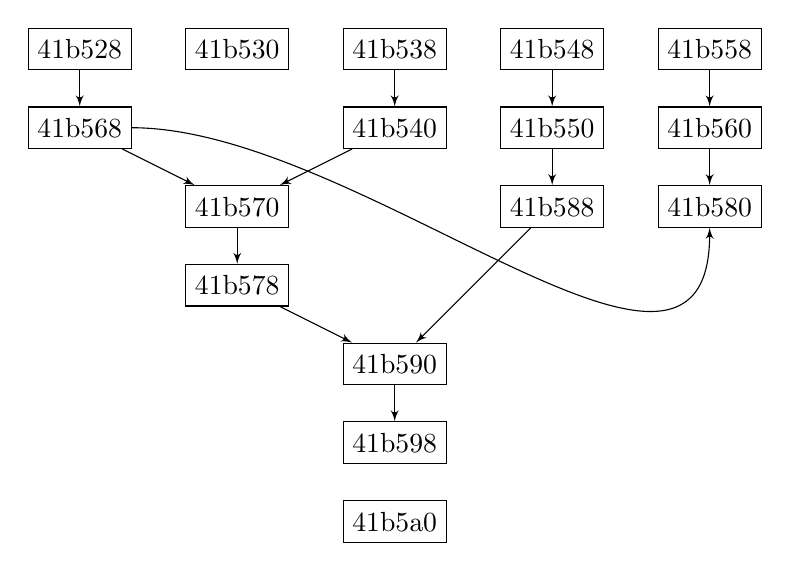
\begin{tikzpicture}
    \tikzset{vertex/.style = {shape=rectangle, draw, minimum size=1.5em}}
    \tikzset{edge/.style = {->,> = latex'}}

    \node[vertex] (41b528) at (0,6) {41b528};
    \node[vertex] (41b530) at (2,6) {41b530};
    \node[vertex] (41b538) at (4,6) {41b538};
    \node[vertex] (41b540) at (4,5) {41b540};
    \node[vertex] (41b548) at (6,6) {41b548};
    \node[vertex] (41b550) at (6,5) {41b550};
    \node[vertex] (41b558) at (8,6) {41b558};
    \node[vertex] (41b560) at (8,5) {41b560};
    \node[vertex] (41b568) at (0,5) {41b568};
    \node[vertex] (41b570) at (2,4) {41b570};
    \node[vertex] (41b578) at (2,3) {41b578};
    \node[vertex] (41b580) at (8,4) {41b580};
    \node[vertex] (41b588) at (6,4) {41b588};
    \node[vertex] (41b590) at (4,2) {41b590};
    \node[vertex] (41b598) at (4,1) {41b598};
    \node[vertex] (41b5a0) at (4,0) {41b5a0};

    \draw[edge] (41b528) to (41b568);
    \draw[edge] (41b538) to (41b540);
    \draw[edge] (41b548) to (41b550);
    \draw[edge] (41b558) to (41b560);
    \draw[edge] (41b568) to (41b570);
    \draw[edge] (41b568) to[out=0, in=270] (41b580);
    \draw[edge] (41b540) to (41b570);
    \draw[edge] (41b570) to (41b578);
    \draw[edge] (41b550) to (41b588);
    \draw[edge] (41b560) to (41b580);
    \draw[edge] (41b578) to (41b590);
    \draw[edge] (41b588) to (41b590);
    \draw[edge] (41b590) to (41b598);
  \end{tikzpicture}
  \caption{Data dependencies between the instructions.}
  \label{fig:dep}
\end{figure}

We first choose to make our architecture with no limit, this design can be seen in table \ref{tab:vliw1}.

\begin{table}[H]
 \caption{When using 3 ALU, 1 MUL, 1 FPU and 5 BAU units.}
  \label{tab:vliw1}
  \scriptsize
  \centering
  \begin{tabular}{|*{10}{C|}}
    \hline
    \multicolumn{3} {|c|} {\bfseries ALU} &
    \multicolumn{1} {c|} {\bfseries MUL} &
    \multicolumn{1} {c|} {\bfseries FPU}  &
    \multicolumn{5} {c|} {\bfseries BAU} \\ \hline 
                {} & {} & {} & {} & {} & {41b528} & {41b530} & {41b538} & {41b548} & {41b558}\\ \hline
                {41b540} & {41b568} & {41b560} & {} & {} & {41b560} & {} & {} & {} & {}\\ \hline
                {41b570} & {41b588} & {41b580} & {} & {} & {} & {} & {} & {} & {}\\ \hline
                {} & {} & {} & {} & {} & {41b578} & {} & {} & {} & {}\\ \hline
                {41b590} & {} & {} & {} & {} & {} & {} & {} & {} & {}\\ \hline
                {} & {} & {} & {} & {} & {41b598} & {41b5a0} & {} & {} & {}\\ \hline
  \end{tabular}
\end{table}
We then tried to reduce some of the units without loosing any performance, we first by tried by removing one of the BAUs (figure \ref{tab:vliw2}), since those are the most expensive units. In table \ref{tab:performance} we can see that this design (VLIW2) doesn't perform any worse than the first design (VLIW1), so we continued to reduce more units to try and get an even cheaper design for this block.

\begin{table}[H]
  \caption{When using 3 ALU, 1 MUL, 1 FPU and 3 BAU units.}
  \label{tab:vliw2}
  \scriptsize
  \centering
  \begin{tabular}{|*{8}{p{8mm}|}}
    \hline
    \multicolumn{3} {|c|} {\bfseries ALU} &
    \multicolumn{1} {c|} {\bfseries MUL} &
    \multicolumn{1} {c|} {\bfseries FPU}  &
    \multicolumn{3} {c|} {\bfseries BAU} \\ \hline 
                {} & {} & {} & {} & {} & {41b528} & {41b558} & {41b538} \\ \hline
                {41b568} & {41b540} & {41b560} & {} & {} & {41b548} & {41b530} & {}\\ \hline
                {41b570} & {41b580} & {} & {} & {} & {41b550} & {} & {} \\ \hline
                {41b588} & {} & {} & {} & {} & {41b578} & {} & {}\\ \hline
                {41b590} & {} & {} & {} & {} & {} & {} & {} \\ \hline
                {} & {} & {} & {} & {} & {41b598} & {41b5a0} & {}\\ \hline
  \end{tabular}
\end{table}

We tried to remove one more BAU, and one ALU (table \ref{tab:vliw3}). In table \ref{tab:performance} we can see that the performance is still the same as in the previous design, even though we have reduced it a lot.

\begin{table}[H]
  \caption{When using 2 ALU, 1 MUL, 1 FPU and 2 BAU units.}
  \label{tab:vliw3}
  \scriptsize
  \centering
  \begin{tabular}{|*{6}{p{8mm}|}}
    \hline
    \multicolumn{2} {|c|} {\bfseries ALU} &
    \multicolumn{1} {c|} {\bfseries MUL} &
    \multicolumn{1} {c|} {\bfseries FPU}  &
    \multicolumn{2} {c|} {\bfseries BAU} \\ \hline 
                {} & {} & {} & {} & {41b528} & {41b538} \\ \hline
                {41b568} & {41b540} & {} & {} & {41b548} & {41b558}\\ \hline
                {41b570} & {41b560} & {} & {} & {41b550} & {41b530} \\ \hline
                {41b588} & {41b580} & {} & {} & {41b578} & {}\\ \hline
                {41b590} & {} & {} & {} & {} & {} \\ \hline
                {} & {} & {} & {} & {41b598} & {41b5a0}\\ \hline
  \end{tabular}
\end{table}

If we take a look in table \ref{tab:pricelist} we can see that the by far most expensive unit is the BAU, and by reducing this from 5 to 2 units we have reduced the price by more than half of the first deigns price. Because of this, we wanted to make sure we weren't able to reduce the design even further, and so we tried using only 1 BAU unit (table \ref{tab:vliw4}).

\begin{table}[H]
  \caption{When using 2 ALU, 1 MUL, 1 FPU and 1 BAU.}
  \label{tab:vliw4}
  \scriptsize
  \centering
  \begin{tabular}{|*{5}{p{8mm}|}}
    \hline
    \multicolumn{2} {|c|} {\bfseries ALU} &
    \multicolumn{1} {c|} {\bfseries MUL} &
    \multicolumn{1} {c|} {\bfseries FPU}  &
    \multicolumn{1} {c|} {\bfseries BAU} \\ \hline 
                {} & {} & {} & {} & {41b528} \\ \hline
                {} & {} & {} & {} & {41b538} \\ \hline
                {41b568} & {41b540} & {} & {} & {41b558} \\ \hline
                {41b570} & {41b560} & {} & {} & {41b548} \\ \hline
                {41b580} & {} & {} & {} & {41b550} \\ \hline
                {41b588} & {} & {} & {} & {41b578} \\ \hline
                {41b590} & {} & {} & {} & {41b530} \\ \hline
                {} & {} & {} & {} & {41b598} \\ \hline
                {} & {} & {} & {} & {41b5a0}\\ \hline
  \end{tabular}
\end{table}

Instead of 6 clock cycles, we now got 9. Which means the design is 50\% worse than the other ones. thus we stopped here.

\begin{table}[H]
  \caption{}
  \label{tab:performance}
  \scriptsize
  \centering
  \begin{tabular}{|*{5}{r|}}
    \hline
        {\bfseries Design} & {\bfseries VLIW1} & {\bfseries VLIW2} & {\bfseries VLIW3} & {\bfseries VLIW4} \\ \hline
        {No. ALU} & {3} & {3} & {2} & {2} \\ \hline
        {No. MUL} & {1} & {1} & {1} & {1} \\ \hline
        {No. FPU} & {1} & {1} & {1} & {1} \\ \hline
        {No. BAU} & {5} & {3} & {2} & {1} \\ \hline
        {Total Cost} & {554} & {354} & {252} & {152} \\ \hline
        {No. Cycles} & {6} & {6} & {6} & {9} \\ \hline
        {Cost per. ratio} & {3324} & {2124} & {1512} & {1368} \\ \hline
  \end{tabular}
\end{table}
The prices for the different units can be seen in table \ref{tab:pricelist}.

\begin{table}[H]
  \caption{}
  \label{tab:pricelist}
  \scriptsize
  \centering
  \begin{tabular}{|*{2}{r|}}
    \hline
    \multicolumn{2} {|c|} {\bfseries Pricelist} \\ \hline
        {\bfseries ALU cost} & {2} \\ \hline
        {\bfseries MUL cost} & {16} \\ \hline
        {\bfseries FPU cost} & {32} \\ \hline
        {\bfseries BAU cost} & {100} \\ \hline
  \end{tabular}
\end{table}

\section{Discussion}
Of course our results are only for one block of code and therefore our design of course might not be a very good one, except here. We choose to use an FPU and an MUL even though they weren't needed in our block, We think that this can be justified by arguing that without these, the design would be completely useless for other code blocks.

We think that the third design (table \ref{tab:vliw3}), is for this block the clear winner.

\newpage
\appendix

\section{Graph file}\label{app:graph}
\begin{lstlisting}
0x0041b528
0x0041b530
0x0041b538
0x0041b548
0x0041b558

0x0041b528 0x0041b568
0x0041b538 0x0041b540
0x0041b548 0x0041b550
0x0041b558 0x0041b560

0x0041b568 0x0041b570
0x0041b540 0x0041b570

0x0041b568 0x0041b580
0x0041b560 0x0041b580

0x0041b570 0x0041b578

0x0041b550 0x0041b588

0x0041b578 0x0041b590
0x0041b588 0x0041b590

0x0041b590 0x0041b598

0x0041b5a0
\end{lstlisting}
\newpage

\section{VLIW files}
\begin{lstlisting}[caption=VLIW 1, basicstyle=\tiny]
3          		         1   1   5
nop        nop        nop        nop nop 0x0041b528 0x0041b530 0x0041b538 0x0041b548 0x0041b558
0x0041b540 0x0041b568 0x0041b560 nop nop 0x0041b550 nop        nop        nop        nop
0x0041b570 0x0041b588 0x0041b580 nop nop nop        nop        nop        nop        nop
nop        nop        nop        nop nop 0x0041b578 nop        nop        nop        nop
0x0041b590 nop        nop        nop nop nop        nop        nop        nop        nop
nop        nop        nop        nop nop 0x0041b598 0x0041b5a0 nop        nop        nop
\end{lstlisting}

\begin{lstlisting}[caption=VLIW 2, basicstyle=\tiny]
3                                1   1   3
nop        nop        nop        nop nop 0x0041b528 0x0041b558 0x0041b538
0x0041b568 0x0041b540 0x0041b560 nop nop 0x0041b548 0x0041b530 nop
0x0041b570 nop        0x0041b580 nop nop 0x0041b550 nop        nop
0x0041b588 nop        nop        nop nop 0x0041b578 nop        nop
0x0041b590 nop        nop        nop nop nop        nop        nop
nop        nop        nop        nop nop 0x0041b598 0x0041b5a0 nop
\end{lstlisting}

\begin{lstlisting}[caption=VLIW 3, basicstyle=\tiny]
2                     1   1   2
nop        nop        nop nop 0x0041b528 0x0041b538
0x0041b568 0x0041b540 nop nop 0x0041b548 0x0041b558
0x0041b570 0x0041b560 nop nop 0x0041b550 0x0041b530
0x0041b588 0x0041b580 nop nop 0x0041b578 nop
0x0041b590 nop        nop nop nop        nop		
nop        nop        nop nop 0x0041b598 0x0041b5a0	
\end{lstlisting}

\begin{lstlisting}[caption=VLIW 4, basicstyle=\tiny]
2                     1   1   1
nop        nop        nop nop 0x0041b528	
nop        nop        nop nop 0x0041b538	
0x0041b568 0x0041b540 nop nop 0x0041b558	
0x0041b570 0x0041b560 nop nop 0x0041b548	
0x0041b580 nop        nop nop 0x0041b550
0x0041b588 nop        nop nop 0x0041b578	
0x0041b590 nop        nop nop 0x0041b530		
nop        nop        nop nop 0x0041b598	
nop        nop        nop nop 0x0041b5a0
\end{lstlisting}
\end{document}

